\documentclass{beamer}
\usepackage[utf8]{inputenc}
\usepackage[T1]{fontenc}

\usebackgroundtemplate{
	
\includegraphics[width=\paperwidth,height=\paperheight]{img/background}
}

\title{Chapter 02: Entity-Relationship Modeling}

\author[P.A. Nugroho]{Pascal Alfadian Nugroho}
\institute[IF-UNPAR]{Program Studi Informatika, \\Universitas Katolik Parahyangan}

\begin{document}
	\begin{frame}
		\titlepage
	\end{frame}

	\section{Introduction}
	\begin{frame}{Introduction}
		\begin{itemize}
			\item Emphasis in structured system analysis is on the \textbf{operations}, rather than \textbf{data}
            \item Entity-relationship Modelling (ERM) is a semiformal data-oriented technique for specifying the product.
            \item Obviously, you can do both for analyzing projects.
		\end{itemize}
	\end{frame}
	\begin{frame}{Introduction}
		\begin{itemize}
			\item The modelling are mostly done using the Entity-Relationship Diagram (ERD)
			\item The benefit, is that it can be easily converted to SQL database tables
            \item Turns out there are so many variations in modelling, and very well described in \cite{song1995}
            \item In this lecture, we are using ``Visual Paradigm'' tool, which is based on TODO notation. The Community Edition is free.
		\end{itemize}
	\end{frame}
	
	\section{Basic Examples of ERD}
	\subsection{Simple Entity-Relationship Diagram}
	\begin{frame}{Simple Entity-Relationship Diagram}
		\begin{columns}[t,totalwidth=\textwidth]
			\column{.5\linewidth}
				\begin{itemize}
					\item This is a simple example of ERD, from \cite{Schach:2006:OCS:1207045} but drawn using Barker (a.k.a. CASE*) notation \cite{barker1992case} 
				\end{itemize}
			\column{.5\linewidth}
				\begin{flushright}
					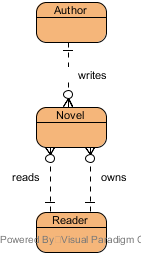
\includegraphics[scale=0.7]{img/02_simple_erd}
				\end{flushright}
		\end{columns}
	\end{frame}
	
	\section{References}
	\begin{frame}[allowframebreaks]
	        \frametitle{References}
	        \bibliographystyle{amsalpha}
	        \bibliography{module_02}
	\end{frame}	
\end{document}

